% !TEX encoding = UTF-8 Unicode

\chapter{Ortografia}

\section{Alfabeto}

\begin{minipage}{0.48\textwidth}
    \begin{table}[H]
        \centering
        \begin{tabular}{lr}
            \toprule
            Scritto     &   Letto \\
            \midrule
            sh          &   \textbf{sci}operare (italiano)\\
            dh          &   \textbf{th}e (inglese) \\
            zh          &   gara\textbf{ge} (francese)\\
            xh          &   \textbf{j}ack (inglese) \\
            gj          &   \textbf{g}ianduia (italiano)\\
            j           &   i (italiano)\\
            q           &   \textbf{c}iao (italiano)\\
            k           &   \textbf{c}asa (italiano)\\ 
            y           &   D\textbf{u} domain (francese)\\
            z           &   ro\textbf{s}a (italiano) \\
            ç           &   \textbf{c}isterna (italiano) \\
            c           &   \textbf{z}ona (italiano) \\
            g           &   \textbf{g}ola \\
            x           &   ca\textbf{s}a (italiano) \\
            \bottomrule
        \end{tabular}
    \end{table}
\end{minipage}\quad%
\begin{minipage}{0.48\textwidth}
    \begin{figure}[H]
        \centering
        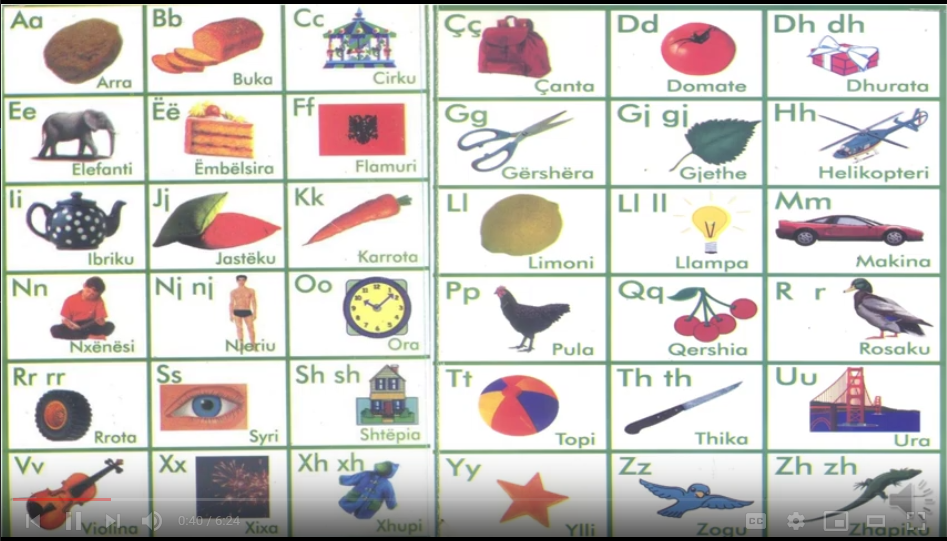
\includegraphics[width=0.8\textwidth]{src/images/alfabetoAlbanese.PNG}
        \caption{Alfabeto albanese}
    \end{figure}
\end{minipage}




\chapter{L'essenziale nella comunicazione base}

\section{Saluti}

\begin{table}[H]
    \centering
    \begin{tabular}{lr}
        \toprule
        Italiano    &   Albanese \\
        \midrule
        \addTranslationRow{Buon Mattino}\\
        \addTranslationRow{Buongiorno}\\
        \addTranslationRow{Buona sera}\\
        \addTranslationRow{Buona notte}\\
        \addTranslationRow{A presto}\\
        \addTranslationRow{Piacere}\\
        \addTranslationRow{Ci vediamo presto}\\
        \addTranslationRow{Arrivederci}\\
        \addTranslationRow{Addio}\\
        \addTranslationRow{Ciao}\\
        \addTranslationRow{Bene}\\
        \bottomrule
    \end{tabular}
\end{table}

\section{Espressioni comuni}

\begin{table}[H]
    \centering
    \begin{tabular}{lr}
        \toprule
        Italiano    &   Albanese \\
        \midrule
        \addTranslationRow{Grazie}\\
        \addTranslationRow{Per favore}\\
        \addTranslationRow{Perdonami}\\
        \addTranslationRow{Mi dispiace}\\
        \addTranslationRow{Come stai?}\\
        \addTranslationRow{Puoi ripeterlo un'altra volta per favore?}\\
        \addTranslationRow{Parlo poco albanese}\\
        \addTranslationRow{Non parlo per niente l'albanese}\\
        \addTranslationRow{Non capisco}\\
        \addTranslationRow{Un momento per favore}\\
        \addTranslationRow{Ti prego, aspetta un minuto}\\
        \addTranslationRow{Si (ok)}\\
        \addTranslationRow{No}\\
        \addTranslationRow{Forse}\\
        \addTranslationRow{Quindi}\\
        \bottomrule
    \end{tabular}
\end{table}

\chapter{Grammatica albanese}

\section{Verbo essere e avere}

\begin{table}[H]
    \centering
    \begin{tabular}{lr}
        \toprule
        Italiano    &   Albanese \\
        \midrule
        Io sono & Unë iam \\
        Tu sei & Ti je\\
        Egli è & Ai është\\
        Ella è & Ajo është\\
        Noi siamo & Ne jemi \\
        Voi siete & Ju jeni \\
        Essi sono & Ata jan \\
        Esse sono & Ato jan \\
        \bottomrule
    \end{tabular}
    \caption{Verbo essere nell'indicativo}
\end{table}

\begin{table}[H]
    \centering
    \begin{tabular}{lr}
        \toprule
        Italiano    &   Albanese \\
        \midrule
        Io sono & Unë kam \\
        Tu sei & Ti ke\\
        Egli è & Ai ka\\
        Ella è & Ajo ka\\
        Noi siamo & Ne kemi \\
        Voi siete & Ju keni \\
        Essi sono & Ata kanë \\
        Esse sono & Ato kanë \\
        \bottomrule
    \end{tabular}
    \caption{Verbo avere nell'indicativo}
\end{table}

\section{Verbi}

Ci sono 3 coniugazioni, che si distinguono per la terminazione dell'infinito presente.

\subsection{Indicativo presente}

\subsubsection{Prima Coniugazione}

Sono verbi il cui infinito termina con \dquote{j}. Le desinenze piàù usuali sono: -oj, -aj, -ej, -ëj, -ij, -yj, -uaj, -yej. Generalmente, in pronuncia, l'accento cade sull'ultima sillaba del tema verbale (\eg{} \textit{punoj} l'accento è messo sulla \dquote{o})\cite{vocedellaquila:verbiprimogruppo, viola:verbiprimogruppo}.

\begin{note}
Proprio come in italiano per la prima coniugazione (\ie{} -are), i verbi del primo gruppo contentono tutti i verbi provenienti dall'esterno\cite{vocedellaquila:verbiprimogruppo}.
\end{note}

\begin{table}[H]
    \centering
    \begin{tabular}{lr|lr|lr}
        \toprule
        Italiano    &   Albanese & Italiano & Albanese & Italiano & Albanese \\
        \midrule
        \addTripleTranslationRow{Andare}{Lavorare}{Imparare}\\
        \addTripleTranslationRow{Vivere}{Cantare}{Leggere}\\
        \addTripleTranslationRow{Scrivere}{Fare}{Ascoltare}\\
        \addTripleTranslationRow{Capire}{Contare}{Dimenticare}\\
        \addTripleTranslationRow{Guardare}{Iniziare}{Finire}\\
        \addTripleTranslationRow{Pulire}{Lavare}{Chiedere}\\
        \addTripleTranslationRow{Correre}{Rompere}{Mordere}\\
        \addTripleTranslationRow{Piangere}{Radere}{Tenere}\\
        \addTripleTranslationRow{Valere}{Vincere}{Girare}\\
        \addTripleTranslationRow{Lodare}{Gioire}{Abitare}\\
        \addTripleTranslationRow{Danneggiare}{Permettere}{Lasciare}\\
        \addTripleTranslationRow{Continuare}{Passare}{Lottare}\\
        \addTripleTranslationRow{Unire}{Credere}{Liberare}\\
        \addTripleTranslationRow{Inviare}{Dubitare}{Ringraziare}\\
        \bottomrule
    \end{tabular}
    \caption{Verbo avere nell'indicativo}
\end{table}

Nella format dell'indicativo presente, i verbi sono coniugati in accordo alla \tblref{bl:verb:primaconiugazione:indicativo:presente}.

\begin{table}[H]
    \centering
    \begin{tabular}{lr}
        \toprule
        Italiano    &   Albanese\\
        \midrule
        Io lavoro           &   Unë puno\textbf{j} \\
        Tu lavori           &   Ti puno\textbf{n} \\
        Egli/Ella lavora    &   Ai/Ajo puno\textbf{n} \\
        Noi lavoriamo       &   Ne puno\textbf{jmë} \\
        Voi lavorate        &   Ju puno\textbf{ni} \\
        Essi/esse lavorano  &   Ata/Ato puno\textbf{jnë} \\
        \bottomrule
    \end{tabular}
    \caption{indicativo presente, prima coniugazione.}
    \label{tbl:verb:primaconiugazione:indicativo:presente}
\end{table}

La stessa tabella è mostrata per il verbo andare (irregolare in italiano ma regolare in albanese).

\begin{table}[H]
    \centering
    \begin{tabular}{lr}
        \toprule
        Italiano    &   Albanese\\
        \midrule
        Io vado           &   Unë shko\textbf{j} \\
        Tu vai           &   Ti shko\textbf{n} \\
        Egli/Ella va    &   Ai/Ajo shko\textbf{n} \\
        Noi andiamo       &   Ne shko\textbf{jmë} \\
        Voi andate        &   Ju shko\textbf{ni} \\
        Essi/esse vanno  &   Ata/Ato shko\textbf{jnë} \\
        \bottomrule
    \end{tabular}
    \caption{indicativo presente, prima coniugazione del verbo andare.}
    \label{tbl:verb:andare:primaconiugazione:indicativo:presente}
\end{table}

\subsubsection{Seconda Coniugazione}

Sono verbi il cui infinito termina con una qualunque consonante. Le più comuni sono \dquote{p}, \dquote{s}, \dquote{l}. Inoltre la radice dei verbi non è tutto l'infinito tranne l'ultima consonanta, ma è possibile che la penultima lettera (solitamente una vocale) sia inclusa nella desinenza). La coniugazione è una delle più irregolari: per questo mostreremo le varie coniugazioni per ogni tempo.

\begin{table}[H]
    \centering
    \begin{tabular}{lr}
        \toprule
        Italiano    &   Albanese \\
        \midrule
        \addTranslationRow{Aprire}\\
        \addTranslationRow{Parlare}\\
        \addTranslationRow{Uscire}\\
        \addTranslationRow{Vendere}\\
        \addTranslationRow{Domandare}\\
        \addTranslationRow{chiamare}\\
        \addTranslationRow{bussare}\\
        \bottomrule
    \end{tabular}
    \caption{Verbi della seconda coniugazione}
\end{table}

A livello generico, la coniugazione segue la seguente forma:

\begin{table}[H]
    \centering
    \begin{tabular}{lr}
        \toprule
        Italiano    &   Albanese\\
        \midrule
        Io          &   forma infinita \\
        Tu          &   forma infinita o \textbf{et} \\
        Egli/Ella   &   format infinita o \textbf{et} \\
        Noi         &   \textbf{im} \\
        Voi         &   \textbf{ni} \\
        Essi/esse   &   \textbf{in} \\
        \bottomrule
    \end{tabular}
    \caption{indicativo presente, seconda coniugazione di un generico verbo. Nella seconda colonna è mostrata la desinenza o, in caso di irregolarità, se è possibile usare anche la forma infinita del verbo.}
    \label{tbl:verb:secondaconiugazione:indicativo:presente}
\end{table}

\begin{table}[H]
    \centering
    \begin{tabular}{lccccccc}
        \toprule
        Pronome     &   Aprire  & Parlare   & Uscire    & Vendere   & Domandare & chiamare & Bussare \\
        \midrule
        Io          &   hap     & flas      & dal       & shes      & pyes  & thërras   & trokas\\
        Tu          &   hap     & flet      & del       & shet      & pyes  & thërret   & troket\\
        Egli/Ella   &   hap     & flet      & del       & shet      & pyes &    thërret & troket\\
        Noi         &   hapim   & flasim    & dalim     & shesim    & pyesim    & thërrasim & trokasim\\
        Voi         &   hapni   & flisni    & dilni     & shisni    &pyesni     & thërrisni & trokisni\\
        Essi/esse   &   hapin   & flasin    & dalin     & shesin    & pyesin    & thërrasin & trokasin\\
        \bottomrule
    \end{tabular}
    \caption{indicativo presente, seconda coniugazione dei verbi hap, flas, dal, shes, pyes, thërras, trokas.}
    \label{tbl:verb:secondaconiugazione:indicativo:presente}
\end{table}

\subsubsection{Terza Coniugazione}

I verbi della terza coniugazione sono quelli i cui infinito termina con una vocale. Tra le vocali ammesse, troviamo \dquote{i}, \dquote{a}, e \dquote{e}. La coniugazione è sicuramente più regolare rispetto alla seconda. A livello generico la coniugazione si comporta come segue:

\begin{table}[H]
    \centering
    \begin{tabular}{lr}
        \toprule
        Italiano    &   Albanese\\
        \midrule
        Io          &   forma infinita \\
        Tu          &   forma infinita\\
        Egli/Ella   &   format infinita\\
        Noi         &   \textbf{më} \\
        Voi         &   \textbf{ni} \\
        Essi/esse   &   \textbf{në} \\
        \bottomrule
    \end{tabular}
    \caption{indicativo presente, seconda coniugazione di un generico verbo. Nella seconda colonna è mostrata la desinenza o, in caso di irregolarità, se è possibile usare anche la forma infinita del verbo.}
    \label{tbl:verb:secondaconiugazione:indicativo:presente}
\end{table}

Una lista dei verbi è disponibile in \tblref{fig:verb:terzacongiugazione}.

\begin{table}[H]
    \centering
    \begin{tabular}{lr}
        \toprule
        Italiano    &   Albanese \\
        \midrule
        \addTranslationRow{Restare}\\
        \addTranslationRow{Dormire}\\
        \addTranslationRow{Bere}\\
        \addTranslationRow{Conoscere}\\
        \addTranslationRow{Mangiare}\\
        \bottomrule
    \end{tabular}
    \caption{Verbi della terza coniugazione}
    \label{fig:verb:terzacongiugazione}
\end{table}

Esempi di come sono coniugati i verbi sono mostrati in \tblref{tbl:verb:terzaconiugazione:indicativo:presente}

\begin{table}[H]
    \centering
    \begin{tabular}{lccccccc}
        \toprule
        Pronome     &   Restare  & Dormire   & Bere    & Conoscere   & Mangiare \\
        \midrule
        Io          &   rri     & fle      & pi       & di      & ha\\
        Tu          &   rri     & fle      & pi       & di      & ha\\
        Egli/Ella   &   rri     & fle      & pi       & di      & ha \\
        Noi         &   rrimë   & flemë    & pimë     & dimë    & hamë \\
        Voi         &   rrini   & fleni    & pini     & dini    & hani \\
        Essi/esse   &   rrinë   & flenë    & pinë     & dinë    & hanë\\
        \bottomrule
    \end{tabular}
    \caption{indicativo presente, seconda coniugazione dei verbi rri, fle, pi, di, ha.}
    \label{tbl:verb:terzaconiugazione:indicativo:presente}
\end{table}

\subsection{Imperfetto}

Nel verbo essere ed avere l'imperfetto è riportato in \tblref{tbl:verb:imperfettto:essereavere}\cite{studylib:imperfetto}.

\begin{table}[H]
    \centering
    \begin{tabular}{lcc}
        \toprule
        Pronome     &   Essere & Avere \\
        \midrule
        Io          &   ish-a & kish-a \\
        Tu          &   ish-e & kish-e \\
        Egli/Ella   &   ish-te & kish-te \\
        Noi         &   ish-im & kish-im \\
        Voi         &   ish-it & kish-it \\
        Essi/esse   &   ish-in & kish-in \\
        \bottomrule
    \end{tabular}
    \caption{imperfetto, verbo essere ed avere.}
    \label{tbl:verb:imperfettto:essereavere}
\end{table}

\begin{table}[H]
    \centering
    \begin{tabular}{lcc}
        \toprule
        Pronome     &   Attivo & Passivo \\
        \midrule
        Io          &   shiko-ja & shiko-hesha \\
        Tu          &   shiko-je & shiko-heshe \\
        Egli/Ella   &   shiko-nte & shiko-hej \\
        Noi         &   shiko-nim & shiko-heshim \\
        Voi         &   shiko-nit & shiko-heshit \\
        Essi/esse   &   shiko-nin & shiko-heshin \\
        \bottomrule
    \end{tabular}
    \caption{imperfetto, prima coniugazione.}
    \label{tbl:verb:primaconiugazione:imperfetto}
\end{table}

\begin{note}
    Nel passivo, la \dquote{h} intervocalica, spezza le due vocali tra fine radice ed inizio della desinenza. Va pronunciata.
\end{note}

\begin{table}[H]
    \centering
    \begin{tabular}{lcc}
        \toprule
        Pronome     &   Attivo & Passivo \\
        \midrule
        Io          &   merr-ja & merr-esha \\
        Tu          &   merr-je & merr-eshe \\
        Egli/Ella   &   merr-te & merr-ej \\
        Noi         &   merr-nim & merr-eshim \\
        Voi         &   merr-nit & merr-eshit \\
        Essi/esse   &   merr-nin & merr-eshin \\
        \bottomrule
    \end{tabular}
    \caption{imperfetto, secondo coniugazione.}
    \label{tbl:verb:primaconiugazione:imperfetto}
\end{table}

A livello generale, se la radice termina con una consonante e la desidenza inizia con la consonante, la \dquote{n} va evitata, poiché è difficile da pronunciare. Infatti nella terza persona \textit{bie} è coniugata con \textit{binte} (nota la n) mentre in \textit{jap} è coniugata (sempre in terza persona) con \textit{japte} (nota la mancata n): non si riesce a pronunciare \textit{japnte}.

Ci sono alcuni verbi della seconda coniugazione che, caso strano, sono sono irregolari anche nell'imperfetto. Vedi \tblref{tbl:verb:secondaconiugazione:imperfetto}.

\begin{table}[H]
    \centering
    \begin{tabular}{lccccccc}
        \toprule
        Pronome     &   Ha      & Rri   & Bie   & Jap   & Shoh      & Vij   & Them \\
        \midrule
        Io          &   ha-ja & rri-ja & bi-ja & jap-ja & shih-ja & vi-ja & thosh-a \\
        Tu          &   ha-je & rri-je & bi-je & jap-je & shih-je & vi-je & thosh-e \\
        Egli/Ella   &   ha-nte & rri-nte & bi-nte & jap-te & shih-te & vi-nte & thosh-te \\
        Noi         &   ha-nim & rri-nim & bi-nim & jap-nin & shih-nim & vi-nim & thosh-im \\
        Voi         &   ha-nit & rri-nit & bi-nit & jap-nit & shih-nit & vi-nit & thosh-it \\
        Essi/esse   &   merr-nin & rri-nin & bi-nin & jap-nin & shih-nin & vi-nin & thosh-in \\
        \bottomrule
    \end{tabular}
    \caption{imperfetto, secondo coniugazione.}
    \label{tbl:verb:secondaconiugazione:imperfetto}
\end{table}

\subsection{Futuro semplice}

Il futuro semplice\cite{vocedellaquila:futurosemplice} è il seguente. A livello generale il futuro è implementato mettendo la particella \textbf{do tё} prima del verbo. La sintassi è la seguente:

\begin{center}
    soggetto + do tё + verbo coniugato
\end{center}

\begin{table}[H]
    \centering
    \begin{tabular}{lcc}
        \toprule
        Pronome     &   Attivo & Passivo \\
        \midrule
        Io          &   la-j & la-hem \\
        Tu          &   la-sh & la-hesh \\
        Egli/Ella   &   la-jё & la-het \\
        Noi         &   la-jmё & la-hemi \\
        Voi         &   la-ni & la-heni \\
        Essi/esse   &   la-jnё & la-hen \\
        \bottomrule
    \end{tabular}
    \caption{futuro semplice, prima coniugazione.}
    \label{tbl:verb:primaconiugazione:futurosemplice}
\end{table}

Nella seconda persona singola, siccome la desinenza è \dquote{sh}: nei verbi della seconda coniugazione (che per definizione terminano in consonante) tra l'ultima lettera consonantica della radice e la prima lettera consonantica della desinenza viene messa una \dquote{ё}

\begin{table}[H]
    \centering
    \begin{tabular}{lcc}
        \toprule
        Pronome     &   Attivo & Passivo \\
        \midrule
        Io          &   hap & hap-em \\
        Tu          &   hap-\textbf{ё}sh & hap-esh \\
        Egli/Ella   &   hap-ё & hap-et \\
        Noi         &   hap-im & hap-emi \\
        Voi         &   hap-ni & hap-eni \\
        Essi/esse   &   hap-in & hap-en \\
        \bottomrule
    \end{tabular}
    \caption{futuro semplice, seconda coniugazione.}
    \label{tbl:verb:primaconiugazione:futurosemplice}
\end{table}


\subsection{Verbo importanti}

\subsubsection{Volere (dua)}

Il verbo è \textit{dua}, che è della seconda coniugazione. Purtroppo.
Volere significa anche \dquote{Amare} in albanese.

\begin{table}[H]
    \centering
    \begin{tabular}{lcc}
        \toprule
        Pronome     &   Indicativo & Imperfetto \\
        \midrule
        Io          &   dua & do-ja \\
        Tu          &   duan & do-je \\
        Egli/Ella   &   duan & do-nte \\
        Noi         &   dua-m & do-nim \\
        Voi         &   duini & do-nit \\
        Essi/esse   &   dua-n & do-nin \\
        \bottomrule
    \end{tabular}
    \caption{imperfetto, secondo coniugazione del verbo volere.}
    \label{tbl:verb:secondaconiugazione:imperfetto}
\end{table}
Il presente di volere è diverso da come è presenter in rete\cite{angjelina}.

\section{Costruzione delle frasi}

\dquote{Tu non hai nessuno} diventa \dquote{Ti \textbf{nuk} ke asnjë}.

Di seguito le forme affermativa, negativa, interrogativa ed interrogativa negativa.

\begin{itemize}
    \item affermativa: soggetto + verbo;
    \item negativa: soggetto + \textbf{nuk} + verbo;
    \item interrogativa: verbo + soggetto?
    \item interrogativa negativa: \textbf{nuk} + verbo + soggetto?
\end{itemize}

\section{Avverbi di frequenza}

A livello di sintassi, gli avverbi di frequenza va messa dopo quella del verbo.

\begin{table}[H]
    \centering
    \begin{tabular}{lr}
        \toprule
        Italiano    &   Albanese \\
        \midrule
        \addTranslationRow{Mai}\\
        \addTranslationRow{Sempre}\\
        \addTranslationRow{di solito}\\
        \addTranslationRow{spesso}\\
        \addTranslationRow{qualche volta}\\
        \addTranslationRow{raramente}\\
        \addTranslationRow{ogni tanto}\\
        \addTranslationRow{ogni}\\
        \bottomrule
    \end{tabular}
    \caption{Avverbi di frequenza}
    \label{fig:verb:avverbi:frequenza}
\end{table}

Se vuoi dire \dquote{x volte al y} dove \dquote{x} è un numero mentre \dquote{y} è un attributo temporale (\eg{} giorno, anno) bisogna dire \dquote{x herë ... në y} dove x e y sono le traduzioni in albanese.

\section{Interrogazioni}

Per dire \glsref{Chi} puoi usare \glsdesc{Chi}. Per esempio \dquote{chi sei?} si può tradurre con \dquote{Kush je?}

Per dire \glsref{Cosa} puoi usare \glsdesc{çfarë} (\eg{} \dquote{Cosa vuoi?} si può tradurre con \dquote{çfarë do?})

\glsref{Come} si traduce con \glsdesc{Come}.
\glsref{Dove} si traduce con \glsdesc{Dove} (Dove sei? si tradure con \dquote{Kui je?})

In generale questi avverbi interrogativi vanno sempre ad inizio frase.

\begin{table}[H]
    \centering
    \begin{tabular}{lr}
        \toprule
        Italiano    &   Albanese \\
        \midrule
        \addTranslationRow{Chi}\\
        \addTranslationRow{Cosa}\\
        \addTranslationRow{Come}\\
        \addTranslationRow{Quando}\\
        \addTranslationRow{Quanto}\\
        \addTranslationRow{Dove}\\
        \addTranslationRow{Perché}\\
        \bottomrule
    \end{tabular}
    \caption{Avverbi interrogativi}
\end{table}

\section{Aggettivi}

\subsection{Aggettivi possessivi}

\begin{table}[H]
    \centering
    \begin{tabular}{lcccc}
        \toprule
        Italiano    &   Sing. Masc. & Sing. Femm.   &  Plu. Masc.   & Plu. Femm.\\
        \midrule
        mio         &   im/i        & ime/e imja    & e mi          & e mia \\
        tuo         &   yt/i        & jote/e jotja  & e tu          & e tua \\
        suo         &   i/e tij/saj & i/e saj       & i/e tij       & i/e saj \\
        nostro      &   ynë         & jonë          & tanë          & tona \\
        vostro      &   juaj        & juaj          & tuaj          & tuaja \\
        loro        &   i tyre      & e tyre        & e tyre        & e tyre \\
        \bottomrule
    \end{tabular}
    \caption{Aggettivi possessivi.}
\end{table}

\subsection{Aggettivi dimostrativi}

\begin{table}[H]
    \centering
    \begin{tabular}{lr|lr}
        \toprule
        Italiano    &   Albanese & Italiano    &   Albanese \\
        \midrule
        \addDoubleTranslationRow{Questo}{Questa} \\
        \addDoubleTranslationRow{Questi}{Queste} \\
        \addDoubleTranslationRow{Quello}{Quella} \\
        \addDoubleTranslationRow{Quelli}{Quelle} \\
        \bottomrule
    \end{tabular}
    \caption{Aggettivi possessivi.}
\end{table}

Cme esempi abbiamo:

\begin{itemize}
    \item Questo ragazzo è simpatico. \dquote{Ky djalë është simpatik};
    \item Queste ragazze sono belle. \dquote{Keto vajza janë të bukura};
    \item Quel ragazzo e alto. \dquote{Ai djalë është i gjatë};
    \item Quelle ragazze sono studentesse. \dquote{Ato vajza janë studente};
\end{itemize}

\section{Preposizioni, congiunzioni e complementi}

Le preposizioni sono le seguenti:

\begin{table}[H]
    \centering
    \begin{tabular}{lr}
        \toprule
        Italiano    &   Albanese \\
        \midrule
        \addTranslationRow[di-it]{di}\\
        \addTranslationRow{a}\\
        \addTranslationRow{da}\\
        \addTranslationRow[in-it]{in}\\
        \addTranslationRow{con}\\
        \addTranslationRow{su}\\
        \addTranslationRow{per}\\
        \addTranslationRow{tra/fra}\\
        \bottomrule
    \end{tabular}
    \caption{Le p}
\end{table}

Quese preposizioni sono solitamente messe dove in italiano verrebbero messe. Per esempio per dire \dquote{io vado a tirana} dico \dquote{Unë shkoj në Tiranë} (lascia perdere che anche Tirana è declinato).

Inoltre è interessante notare che mentre in italiano esistono 2 preposizioni \dquote{a} e \dquote{in} (per differenziare lo stato in luogo e moto al luogo), in albanese non c'è differenza tra le 2 e vengono entrambe tradotte con \glsdesc{in-it}.

Particolare attenzione va fatta alla preposizione \dquote{di}. Bisogna tradurre:

\begin{itemize}
    \item \dquote{di} con \dquote{i} quando il sostantivo che viene specificato dal complemento di specificazione è maschile;
    \item \dquote{di} con \dquote{e} quando il sostantivo che viene specificato dal complemento di specificazione è femminile;
\end{itemize}

Considera il seguente esempi: \dquote{il libro di Viola} e \dquote{il quaderno di Viola}. il Libro è \glsdesc{Libro} (in albanese maschile) mentre il Quaderno è \glsdesc{Quaderno} (in alòbanese femminile). La prima frase è tradotta con \dquote{Libri i Violës} (perché libri è maschile) mentre la seconda è tradotta con \dquote{Fletorja e Violës} (perché il quaderno è femminile): Il genere del complemento di specificazione (in questo caso Viola) non è coinvolto nella regola.

Ora, la domanda è: se io in italiano voglio usare un complemento, come lo dico in albanese? \tblref{tbl:complementi} ci dice cosa dobbiamo fare per esprimere un complemento in albanese


\begin{table}[H]
    \centering
    \begin{tabular}{lcr}
        \toprule
        Italiano            & Domanda                   & Albanese \\
        \midrule
        \textbf{Oggetto}              & Chi? Che cosa?               &\\
        \textbf{Specificazione}      & Di chi? Di cosa?              &\\
        \textbf{termine}             & A chi? A cosa?                &\\
        \textbf{agente}              & in passivo: Da chi?           & ablativo \\
        \textbf{causa}               & per quale motivo?             & ablativo\\
        \textbf{stato in luogo}      & dove? in che luogo?           & ablativo në\\
        \textbf{moto a luogo}        & verso dove?                   & nominativo (in latino viene usato l'accusativo)\\
        \textbf{moto da luogo}       & da dove?                      & ablativo\\
        \textbf{moto per luogo}      & attraverso dove?              & dativo \\
        \textbf{tempo}               & quando?                       & ablativo \\
        \textbf{fine}                & al fine di chi? a che scopo?  & ablativo (in latino si usa il dativo) \\
        \textbf{mezzo/modo}          & per mezzo di chi? di che cosa?& në dativo (in latino si usa l'ablativo) \\
        \textbf{compagnia}           & con chi? con che cosa?        & accusativo (in latino si usa ablativo) më \\
        \textbf{argomento}           & riguardo cosa?                & accusativo (in latino si usa l'ablativo) \\
        causa efficiente    & da chi? da cosa?              &\\
        prezzo              & per quanto?                   &\\
        abbondanza          & di che cosa?                  &\\
        unione              & con cosa?                     &\\
        qualità             & con quali caratteristiche?    &\\
        materia             & di cosa è composto?           & ablativo\\
        
        vantaggio           & In favore di chi? Di cosa?    &\\
        denominazione       & Di chi? Di cosa?              &\\
        limitazione         & relativamente a che cosa?     &\\
        provenienza         & da dove? da che cosa?         &\\
        paragone            & più o meno di chi? di cosa?   &\\
        età                 & a che età?                    &\\
        quantità            & in che quantità               &\\
        \bottomrule
    \end{tabular}
    \caption{Complementi}
    \label{tbl:complementi}
\end{table}

\section{Numeri}

\begin{note}
    L'albanese con i numero funziona tipo il francese: al posto di dire quaranta, usano 2 venti (proprio come in francese per dire 80 dicono quattro volte venti).
\end{note}

\begin{table}[H]
    \centering
    \begin{tabular}{lr|lr}
        \toprule
        Italiano     &   Albanese & Italiano     &   Albanese \\
        \midrule
        \addDoubleTranslationRow{Numero}{Zero}\\
        \addDoubleTranslationRow{Uno}{Due}\\
        \addDoubleTranslationRow{Tre}{Quattro}\\
        \addDoubleTranslationRow{Cinque}{Sei}\\
        \addDoubleTranslationRow{Sette}{Otto}\\
        \addDoubleTranslationRow{Nove}{Dieci}\\
        \addDoubleTranslationRow{Undici}{Dodici}\\
        \addDoubleTranslationRow{Tredici}{Quattordici}\\
        \addDoubleTranslationRow{Quindici}{Sedici}\\
        \addDoubleTranslationRow{Diciasette}{Diciotto}\\
        \addDoubleTranslationRow{Diciannove}{Venti}\\
        \addDoubleTranslationRow{Ventuno}{Ventidue}\\
        \addDoubleTranslationRow{Ventitre}{Ventiquattro}\\
        \addDoubleTranslationRow{Trenta}{Trentuno}\\
        \addDoubleTranslationRow{Trentadue}{Trentatre}\\
        \addDoubleTranslationRow{Trentaquattro}{Quaranta}\\
        \addDoubleTranslationRow{Cinquanta}{Sessanta}\\
        \addDoubleTranslationRow{Settanta}{Ottanta}\\
        \addDoubleTranslationRow{Novanta}{Cento}\\
        \addDoubleTranslationRow{Mille}{Centomila}\\
        \addDoubleTranslationRow{Un milione}{Dieci milioni}\\
        \bottomrule
    \end{tabular}
\end{table}

\section{Declinazioni}

Proprio come in latino, anche l'albanese possiede delle declinazioni.
A differenza del latino, però, l'albanese declina le parola non solo a seconda del caso, ma anche se si riferisce alla forma determinata o in un modo indeterminato. Se ti serve parlare con un albanese riguardo i casi, essi sono tradotti come in tabella \tblref{tbl:casi:01}\cite{angjelina}.

\begin{table}[H]
    \centering
    \begin{tabular}{lr}
        \toprule
        Italiano & Albanese \\
        \midrule
        \addTranslationRow{Nominativo}\\
        \addTranslationRow{Genitivo}\\
        \addTranslationRow{Dativo}\\
        \addTranslationRow{Accusativo}\\
        \addTranslationRow{Ablativo}\\
        \bottomrule
    \end{tabular}
    \caption{Traduzione dei casi}
    \label{tbl:casi:01}
\end{table}

In generale\cite{ccanta2017category}:

\begin{itemize}
    \item nominativo: per i soggetti;
    \item genitivo: per il complemento di specificazione;
    \item dativo: per complementi come il termine e modo a luogo;
    \item accusativo: complementi oggetti;
    \item ablativo: complementi moto da luogo, stato luogo, agente;
\end{itemize}

\subsection{Declinazione I}

La prima declinazione (\ie{} in latino sarebbe la seconda declinazione) rappresenta la declinazione dei nomi maschili ed include tutti i nomi il cui nominativo determinato termina in \dquote{i}. Per esempio \glsdesc{Mare} è il mare.

\begin{table}[H]
    \centering
    \begin{tabular}{cllll}
        \toprule
        caso        & Ind. Sing.         & Ind. Plu.        & Det. Sing.      & Det. Plu. \\
        \midrule
        Nominativo  & <rad-sing>         & <rad-plu>        & <rad-sing>-i    & <rad-plu>-t  \\
        Genitivo    & <rad-sing>-i       & <rad-plu>-ve     & <rad-sing>-it   & <rad-plu>-ve \\
        Dativo      & <rad-sing>-i       & <rad-plu>-ve     & <rad-sing>-it   & <rad-plu>-ve \\
        Accusativo  & <rad-sing>         & <rad-plu>        & <rad-sing>-in   & <rad-plu>-t \\
        Ablativo    & <rad-sing>-i       & <rad-plu>-sh     & <rad-sing>-it   & <rad-plu>-ve \\
        \bottomrule
    \end{tabular}
    \caption{Declinazione dei maschili. \textit{Det.}(\textit{Ind.}) si riferisce alla forma determinata (indeterminata). \textit{Sing.}(\textit{Plu.}) indica la forma Singolare (Plurale). rad-sing rappresenta la radice singolare mentre rad-plu quella plurale\cite{shqipe-gramatike-01}.}
    \label{decl:1:generale}
\end{table}

In generale, ogni nome ha un nominativo singolare e plurale che vanno ricordati praticamente a memoria. \tblref{decl:1:det} è l'esempio del Mare (\glsdesc{Mare}):

\begin{table}[H]
    \centering
    \begin{tabular}{cllll}
        \toprule
        caso        & Ind. Sing.         & Ind. Plu.        & Det. Sing.      & Det. Plu. \\
        \midrule
        Nominativo  & det         & deta        & det-i    & deta-t  \\
        Genitivo    & det-i       & deta-ve     & det-it   & deta-ve \\
        Dativo      & det-i       & deta-ve     & det-it   & deta-ve \\
        Accusativo  & det         & deta        & det-in   & deta-t \\
        Ablativo    & det-i       & deta-sh     & det-it   & deta-ve \\
        \bottomrule
    \end{tabular}
    \caption{Declinazione dei maschili. \textit{Det.}(\textit{Ind.}) si riferisce alla forma determinata (indeterminata). \textit{Sing.}(\textit{Plu.}) indica la forma Singolare (Plurale). rad-sing rappresenta la radice singolare mentre rad-plu quella plurale.}
    \label{decl:1:det}
\end{table}

Nella tabella \tblref{decl:1:lista} sono presenti alcuni nomi apaprtenenti alla prima declinazione:

\begin{table}[H]
    \centering
    \begin{tabular}{cll}
        \toprule
        Nome        & Nopminativo. Sing.    & Nominativo. Plu.\\
        \midrule
        mare        & det                   & deta \\
        matita      & laps                  & laps \\
        mountain    & mal                   & male \\
        stato       & shtet                 & shtete \\    
        \bottomrule
    \end{tabular}
    \caption{Lista di alcuni nomi apaprtenenti alla prima declinazione.}
    \label{decl:1:lista}
\end{table}

se è della declinazione feminile da a -> e con i 2 punti;
se è della declinazione maschile da o -> i
se è della declinazione maschile da peshk -> peshq


In generale, se la forma indeterminata finisce per \dquote{g,h,k}, la desinenza non è \dquote{i}, ma \dquote{u}.

\subsection{Declinazione II}

La declinazione maschile (\ie{} in latino sarebbe la seconda declinazione) rappresenta la declinazione dei nomi maschili ed include tutti i nomi il cui nominativo determinato termina in \dquote{i}. Per esempio \glsdesc{Mare} è il mare.

\begin{table}[H]
    \centering
    \begin{tabular}{cllll}
        \toprule
        caso        & Ind. Sing.         & Ind. Plu.        & Det. Sing.      & Det. Plu. \\
        \midrule
        Nominativo  & <rad-sing>         & <rad-plu>        & <rad-sing>-u    & <rad-plu>-t  \\
        Genitivo    & <rad-sing>-u       & <rad-plu>-ve     & <rad-sing>-ut   & <rad-plu>-ve \\
        Dativo      & <rad-sing>-u       & <rad-plu>-ve     & <rad-sing>-ut   & <rad-plu>-ve \\
        Accusativo  & <rad-sing>         & <rad-plu>        & <rad-sing>-un   & <rad-plu>-t \\
        Ablativo    & <rad-sing>-u       & <rad-plu>-sh     & <rad-sing>-ut   & <rad-plu>-ve \\
        \bottomrule
    \end{tabular}
    \caption{Declinazione dei mscahili. \textit{Det.}(\textit{Ind.}) si riferisce alla forma determinata (indeterminata). \textit{Sing.}(\textit{Plu.}) indica la forma Singolare (Plurale).}
\end{table}

Alcuni sostantivi hanno il nominativo che terminano con \dquote{-u}. Per esempio Amico (\toAlbanian{Amico}) or Pesce (vedi \tblref{tbl:peshk})

\begin{table}[H]
    \centering
    \begin{tabular}{cllll}
        \toprule
        caso        & Ind. Sing.    & Ind. Plu. & Det. Sing.    & Det. Plu. \\
        \midrule
        Nominativo  & peshk         & -         & peshk-u       & peshk-ut \\
        Genitivo    & & & & \\
        Dativo      & & & & \\
        Accusativo  & & & & \\
        Ablativo    & & & & \\
        \bottomrule
    \end{tabular}
    \caption{Declinazione dei mscahili il cui nominativo indeterminativo termina con una consonante variante. \textit{Det.}(\textit{Ind.}) si riferisce alla forma determinata (indeterminata). \textit{Sing.}(\textit{Plu.}) indica la forma Singolare (Plurale).}
    \label{tbl:peshk}
\end{table}

Consideriamo infine per esempio il termine Ragazzo (\toAlbanian{Ragazzo}), in \tblref{tbl:djale}.

\begin{table}[H]
    \centering
    \begin{tabular}{cllll}
        \toprule
        caso        & Ind. Sing.    & Ind. Plu. & Det. Sing.    & Det. Plu. \\
        \midrule
        Nominativo  & djal-ë         & djem      & djal-i         & djem-të \\
        Genitivo    & djali         & djemve    & djalit        & djemve \\
        Dativo      & djali         & djemve    & djalit        & djemve \\
        Accusativo  & djalë         & djem      & djalin        & djemtë \\
        Ablativo    & djali         & djemsh    & djalit        & djemve \\
        \bottomrule
    \end{tabular}
    \caption{Declinazione di Ragazzo \toAlbanian{Ragazzo}. \textit{Det.}(\textit{Ind.}) si riferisce alla forma determinata (indeterminata). \textit{Sing.}(\textit{Plu.}) indica la forma Singolare (Plurale)\cite{slide:grammatica}.}
    \label{tbl:djale}
\end{table}

Ci sono alcuni nomi la cui forma indeterminata singolare che terminano con una vocale, per esempio Occhio (\toAlbanian{Occhio}): in questo caso è necessario inserire una \dquote{r} tra la radice e la desinenza. Vedi \tblref{tbl:sy}.


\begin{table}[H]
    \centering
    \begin{tabular}{cllll}
        \toprule
        caso        & Ind. Sing.    & Ind. Plu. & Det. Sing.    & Det. Plu. \\
        \midrule
        Nominativo  & sy            & -      & sy-ri         & - \\
        Genitivo    &          &     &         &  \\
        Dativo      &          &     &         &  \\
        Accusativo  &          &       &         &  \\
        Ablativo    &          &     &         &  \\
        \bottomrule
    \end{tabular}
    \caption{Declinazione di Occhio \toAlbanian{Occhio}. \textit{Det.}(\textit{Ind.}) si riferisce alla forma determinata (indeterminata). \textit{Sing.}(\textit{Plu.}) indica la forma Singolare (Plurale)\cite{slide:grammatica}.}
    \label{tbl:sy}
\end{table}

Ci sono poi altri nomi il cui nominativo singolare indeterminato termina con \dquote{-ër}: vedi \tblref{tbl:liber}. In questo caso nel nominativo singolare determinato cade la \dquote{ë}

\begin{table}[H]
    \centering
    \begin{tabular}{cllll}
        \toprule
        caso        & Ind. Sing.    & Ind. Plu. & Det. Sing.    & Det. Plu. \\
        \midrule
        Nominativo  & libër            & -      & libri-ri         & - \\
        Genitivo    &          &     &         &  \\
        Dativo      &          &     &         &  \\
        Accusativo  &          &       &         &  \\
        Ablativo    &          &     &         &  \\
        \bottomrule
    \end{tabular}
    \caption{Declinazione di Occhio \toAlbanian{Occhio}. \textit{Det.}(\textit{Ind.}) si riferisce alla forma determinata (indeterminata). \textit{Sing.}(\textit{Plu.}) indica la forma Singolare (Plurale)\cite{slide:grammatica}.}
    \label{tbl:liber}
\end{table}

Per completezza, ecco la declinazione di un nome generico della seconda declinazione: In \tblref{tbl:mal} questa è la declinazione di Monte (\toAlbanian{Monte}).

\begin{table}[H]
    \centering
    \begin{tabular}{cll|ll}
        \toprule
        caso        & Ind. Sing.    & Ind. Plu. & Det. Sing.    & Det. Plu. \\
        \midrule
        Nominativo  & mal         & mal-e     & mal-i          & mal-et \\
        Genitivo    &          &     &         & \\
        Dativo      &          &     &         & \\
        Accusativo  & mal         & mal-e    & mal-in        & mal-et\\
        Ablativo    &          &     &         & \\
        \bottomrule
    \end{tabular}
    \caption{Declinazione di Ragazzo \toAlbanian{Ragazzo}. \textit{Det.}(\textit{Ind.}) si riferisce alla forma determinata (indeterminata). \textit{Sing.}(\textit{Plu.}) indica la forma Singolare (Plurale)\cite{vocedellaquila:accusativo}.}
    \label{tbl:mal}
\end{table}


\subsubsection{Come determinare il nominativo indeterminato plurale?}

Prima di tutto, alcune regole generali.

Se un sostantivo rappresenta un concetto astratto (come la pazienza, l'errore, il ricordo), e il nominativo indeterminato singolare termina con \dquote{-im}, allora il nominativo plurale indeterminato sarà sempre calcolato aggiungendo \dquote{e} al nominativo indeterminato singolare. Per esempio Pazienza \toAlbanian{Pazienza} diventa \dquote{Durime}.

Se un sostantivo ha il nominativo indeterminato singolare che ha un accento sull'ultima sillaba (\eg{} -ar, -or, -ur), allora il nominativo indeterminato plurale aggiunge la \dquote{-ë} al nominativo indeterminato singolare. Per esempio il Soldato (\toAlbanian{Soldato}) diventa \dquote{Ushtarë}(notare che \toAlbanian{Soldato} termina con una sillaba su cui viene posto l'accento, in questo caso \dquote{ar}).

Ci sono poi delle euristiche per capire quale sia il nominativo indeterminato plurale:

\begin{itemize}
    \item Aggiungendo la desinenza \dquote{-a}. Per esempio (Passo) \toAlbanian{Passo} diventa \dquote{çapa};
    \item Aggiungendo la desinenza \dquote{-e}. Per esempio (Mare) \toAlbanian{Mare} diventa \dquote{deti};
    \item Aggiungendo la desinenza \dquote{-ë}. Per esempio (Soldato) \toAlbanian{Soldato} diventa \dquote{ushtarë};
    \item Aggiungendo la desinenza \dquote{-nj}. Per esempio (Pastore) \toAlbanian{Pastore} diventa \dquote{barinj};
    \item Aggiungendo la desinenza \dquote{-ra}. Per esempio (Villaggio) \toAlbanian{Villaggio} diventa \dquote{fshatra};
    \item Aggiungendo la desinenza \dquote{-ëe}. Per esempio (Genitore) \toAlbanian{Genitore} diventa \dquote{prindër};
    \item Lasciando il plurale identico al singolare. Per esempio (Cane) \toAlbanian{Cane} diventa \dquote{qen};
\end{itemize}

Ci sono infine poi alcuni nomi che sono irregolari e basta e vanno imparati a memoria:

\begin{itemize}
    \item Papà: \toAlbanian{Papà} il cui plurale indeterminato è \dquote{baballarë};
    \item Zio: \toAlbanian{Zio} il cui plurale indeterminato è \dquote{dajllarë};
    \item Ragazzo: \toAlbanian{Ragazzo} il cui plurale indeterminato è \dquote{djem};
    \item Dito: \toAlbanian{Dito} il cui plurale indeterminato è \dquote{gishtërinj};
    \item Persona: \toAlbanian{Persona} il cui plurale indeterminato è \dquote{njerëz};
    \item Fratello: \toAlbanian{Fratello} il cui plurale indeterminato è \dquote{vëllezër};
\end{itemize}


\subsection{Declinazione dei sostantivi femminili}

La declinazione del femminile comprende i nomi che terminano con \dquote{ë}, con una \dquote{i} \textbf{accentata} o con una \dquote{e}. Partiamo con i femminili il cui nominativo indeterminativo singolare terminano con \dquote{ë} (\tblref{tbl:terminacone}). La casistica totale dei nominativi indeterminati singolari è:

\begin{itemize}
    \item terminano con \dquote{-ë};
    \item terminano con \dquote{-i} accentata;
    \item terminano con \dquote{-e} sonora;
    \item terminano con \dquote{-ër};
\end{itemize}

\begin{table}[H]
    \centering
    \begin{tabular}{cllll}
        \toprule
        caso        & Ind. Sing.    & Ind. Plu. & Det. Sing.    & Det. Plu. \\
        \midrule
        Nominativo  & nat-ë         &           & nat-a         & nat-ë  \\
        Genitivo    & & & & \\
        Dativo      & & & & \\
        Accusativo  & & & & \\
        Ablativo    & & & & \\
        \bottomrule
    \end{tabular}
    \caption{Declinazione dei femminili quando il nominativo indeterminato termina con \dquote{-ë}. Il nome coinvolt è Notte (\toAlbanian{Notte}). \textit{Det.}(\textit{Ind.}) si riferisce alla forma determinata (indeterminata). \textit{Sing.}(\textit{Plu.}) indica la forma Singolare (Plurale).}
    \label{tbl:terminacone}
\end{table}

Consideriamo poi il nome che termina con \dquote{-i} accentata. Vediamo tabella \tblref{tbl:terminaconi}.

\begin{table}[H]
    \centering
    \begin{tabular}{cllll}
        \toprule
        caso        & Ind. Sing.    & Ind. Plu. & Det. Sing.    & Det. Plu. \\
        \midrule
        Nominativo  & bukur-i       &       & bukur-ia               &  \\
        Genitivo    & & & & \\
        Dativo      & & & & \\
        Accusativo  & & & & \\
        Ablativo    & & & & \\
        \bottomrule
    \end{tabular}
    \caption{Declinazione dei femminili quando il nominativo indeterminato termina con \dquote{-i}. Il nome coinvolt è Bellezza (\toAlbanian{Bellezza}). \textit{Det.}(\textit{Ind.}) si riferisce alla forma determinata (indeterminata). \textit{Sing.}(\textit{Plu.}) indica la forma Singolare (Plurale).}
    \label{tbl:terminaconi}
\end{table}

Guardiamo poi il gruppo di nomi il cui nominativo indefinito singolare termina con la vocale sonora \dquote{e}.

\begin{table}[H]
    \centering
    \begin{tabular}{cllll}
        \toprule
        caso        & Ind. Sing.    & Ind. Plu. & Det. Sing.    & Det. Plu. \\
        \midrule
        Nominativo  & dritar-e          &       & dritar-ja               &  \\
        Genitivo    & & & & \\
        Dativo      & & & & \\
        Accusativo  & & & & \\
        Ablativo    & & & & \\
        \bottomrule
    \end{tabular}
    \caption{Declinazione dei femminili quando il nominativo indeterminato termina con \dquote{-e}. Il nome coinvolt è Finestra (\toAlbanian{Finestra}). \textit{Det.}(\textit{Ind.}) si riferisce alla forma determinata (indeterminata). \textit{Sing.}(\textit{Plu.}) indica la forma Singolare (Plurale).}
    \label{tbl:terminaconi}
\end{table}

Esistono poi dei nomi femminili che terminano con \dquote{-ër}. La casistica è quella in \tblref{tbl:terminaconer}.

\begin{table}[H]
    \centering
    \begin{tabular}{cllll}
        \toprule
        caso        & Ind. Sing.    & Ind. Plu. & Det. Sing.    & Det. Plu. \\
        \midrule
        Nominativo  & mot-ër        &       & mot-ra               &  \\
        Genitivo    & & & & \\
        Dativo      & & & & \\
        Accusativo  & & & & \\
        Ablativo    & & & & \\
        \bottomrule
    \end{tabular}
    \caption{Declinazione dei femminili quando il nominativo indeterminato termina con \dquote{-ër}. Il nome coinvolta è Madre (\toAlbanian{Madre}). \textit{Det.}(\textit{Ind.}) si riferisce alla forma determinata (indeterminata). \textit{Sing.}(\textit{Plu.}) indica la forma Singolare (Plurale).}
    \label{tbl:terminaconer}
\end{table}

\subsection{Determinazione dell'indeterminato plurale}

Come nella declinazione del maschile, anche il nominativo femminile indeterminato plurale non ha regole fisse. Partiamo da alcune 

\subsection{Complimenti}

L'ablativo viene usato quando non devi usare né un complemento di specificazione né uno di termine (o comunque né il genitivo né il dativo)\cite{vocedellaquila:ablativo}.
A differenza dell'accusativo, genitivo e dativo, l'ablativo è praticamente un contenitore dove mettere tutti gli altri complementi (un pò come il latino, grosso modo): per esempio, come in latino, l'albanese usa l'albativo per i complementi di moto da luogo, d'agente, mezzo, stato in luogo.
Siccome ci sono tanti complementi, l'ablativo è preposto da delle preposizioni per suggerire quali sono   



\chapter{Lessico Generico}

\section{Corpo umano}

\begin{table}[H]
    \centering
    \begin{tabular}{lr}
        \toprule
        Italiano    &   Albanese \\
        \midrule
        \addTranslationRow{Mano} \\
        \addTranslationRow{Denti} \\
        \addTranslationRow{Bocca} \\
        \addTranslationRow{Occhio} \\
        \addTranslationRow{Pancia} \\
        \addTranslationRow{Capelli} \\
        \addTranslationRow{Naso} \\
        \addTranslationRow{Orecchio} \\
        \addTranslationRow{Labbra} \\
        \addTranslationRow{Guancia} \\
        \addTranslationRow{Mento} \\
        \addTranslationRow{Fronte} \\
        \addTranslationRow{Ciglia} \\
        \addTranslationRow{Soppraciglia} \\
        \addTranslationRow{Spalle} \\
        \addTranslationRow{Torace} \\
        \addTranslationRow{Ombelico} \\
        \addTranslationRow{Schiena} \\
        \addTranslationRow{Braccio} \\
        \addTranslationRow{Dito} \\
        \addTranslationRow{Unghie} \\
        \addTranslationRow{Gamba} \\
        \addTranslationRow{Coscia} \\
        \addTranslationRow{Ginocchio} \\
        \addTranslationRow{Polpaccio} \\
        \addTranslationRow{Caviglia} \\
        \addTranslationRow{Glutei} \\
        \bottomrule
    \end{tabular}
    \caption{Lessico riguardo il corpo umano.}
\end{table}

\section{Abitazione}

\begin{table}[H]
    \centering
    \begin{tabular}{lr}
        \toprule
        Italiano    &   Albanese \\
        \midrule
        \addTranslationRow{Casa}\\
        \addTranslationRow{Televisione}\\
        \addTranslationRow{Frigorifero}\\
        \addTranslationRow{Finestra}\\
        \addTranslationRow{Porta}\\
        \addTranslationRow{Divano}\\
        \addTranslationRow{Tavola}\\
        \addTranslationRow{Forno}\\
        \addTranslationRow{Lampada}\\
        \addTranslationRow{Fiore}\\
        \bottomrule
    \end{tabular}
    \caption{Lessico riguardo l'abitazione.}
\end{table}


\section{Colori}

\begin{table}[H]
    \centering
    \begin{tabular}{lr}
        \toprule
        Italiano    &   Albanese \\
        \midrule
        \addTranslationRow{Rosso}\\
        \addTranslationRow{Arancione}\\
        \addTranslationRow{Giallo}\\
        \addTranslationRow{Verde}\\
        \addTranslationRow{blu}\\
        \addTranslationRow{Viola}\\
        \addTranslationRow{rosa}\\
        \addTranslationRow{Bianco}\\
        \addTranslationRow{Marrone}\\
        \addTranslationRow{Grigio}\\
        \addTranslationRow{Nero}\\
        \addTranslationRow{Nera}\\
        \bottomrule
    \end{tabular}
\end{table}


\section{Giorni della settimana, mesi e stagioni}

\begin{table}[H]
    \centering
    \begin{tabular}{lr}
        \toprule
        Italiano    &   Albanese \\
        \midrule
        \addTranslationRow{Sera}\\
        \addTranslationRow{Giorno}\\
        \addTranslationRow{Settimana}\\
        \addTranslationRow{Mese}\\
        \addTranslationRow{Anno}\\
        \addTranslationRow{Stagione}\\
        \addTranslationRow{Primavera}\\
        \addTranslationRow{Estate}\\
        \addTranslationRow{Autunno}\\
        \addTranslationRow{Inverno}\\
        \addTranslationRow{Finesettimana}\\
        \addTranslationRow{Lunedì}\\
        \addTranslationRow{Martedì}\\
        \addTranslationRow{Mercoledì}\\
        \addTranslationRow{Giovedì}\\
        \addTranslationRow{Venerdì}\\
        \addTranslationRow{Sabato}\\
        \addTranslationRow{Domenica}\\
        \addTranslationRow{Gennaio}\\
        \addTranslationRow{Febbraio}\\
        \addTranslationRow{Marzo}\\
        \addTranslationRow{Aprile}\\
        \addTranslationRow{Maggio}\\
        \addTranslationRow{Giugno}\\
        \addTranslationRow{Luglio}\\
        \addTranslationRow{Agosto}\\
        \addTranslationRow{Settembre}\\
        \addTranslationRow{Ottobre}\\
        \addTranslationRow{Novembre}\\
        \addTranslationRow{Dicembre}\\
        \bottomrule
    \end{tabular}
\end{table}

\section{A tavola}

\begin{table}[H]
    \centering
    \begin{tabular}{lr}
        \toprule
        Italiano    &   Albanese \\
        \midrule
        \addTranslationRow{Pasta}\\
        \addTranslationRow{Risotto}\\
        \bottomrule
    \end{tabular}
    \caption{Primi}
\end{table}

\begin{table}[H]
    \centering
    \begin{tabular}{lr}
        \toprule
        Italiano    &   Albanese \\
        \midrule
        \addTranslationRow{Branzino}\\
        \addTranslationRow{Gamberetti}\\
        \addTranslationRow{Gamberi}\\
        \bottomrule
    \end{tabular}
    \caption{Pesci}
\end{table}

\begin{table}[H]
    \centering
    \begin{tabular}{lr}
        \toprule
        Italiano    &   Albanese \\
        \midrule
        \addTranslationRow{Oliva}\\
        \addTranslationRow{Pomodoro}\\
        \addTranslationRow{Cetriolo}\\
        \addTranslationRow{Tuship}\\
        \bottomrule
    \end{tabular}
    \caption{Verdura}
\end{table}


\begin{table}[H]
    \centering
    \begin{tabular}{lr}
        \toprule
        Italiano    &   Albanese \\
        \midrule
        \addTranslationRow{Caffe}\\
        \addTranslationRow{Acqua}\\
        \addTranslationRow{te}\\
        \bottomrule
    \end{tabular}
    \caption{Bevande}
\end{table}


\begin{table}[H]
    \centering
    \begin{tabular}{lr}
        \toprule
        Italiano    &   Albanese \\
        \midrule
        \addTranslationRow{Toilet}\\
        \bottomrule
    \end{tabular}
    \caption{Luoghi}
\end{table}

% \begin{table}[ht]
%     \centering
%     \begin{tabular}{lr}
%         \toprule
%         Italiano    &   Albanese \\
%         \midrule
%         \bottomrule
%     \end{tabular}
% \end{table}
